%%%%%%%%%%%%%%%%%  Debut du fichier Latex  %%%%%%%%%%%%%%%%%%%%%%%%%%%%%%
\documentclass[
    a4paper, 12pt, onecolumn,
    %draft
]{article}

%%% Pour un texte en francais
\usepackage[francais]{babel}
%\usepackage[T1]{fontenc}       % cesure des mots avec accents
\usepackage[latin1]{inputenc}  % encodage des lettres accentuees
                               % pour taper directement ??????? au lieu de \'e

\usepackage{graphicx}
\usepackage[round]{natbib}

%%% Raccourci pour la mise en page
\newcommand{\rubrique}[1]{\bigskip \noindent {\bf #1}}

%%%%%%%%%%%%%%%%%%%%%%%%%%%%%%%%%%%%%%%%%%%%%%%%%%%%%%%%%%%%%%%%%
%%% REMPLACER LES INDICATIONS ENTRE CROCHETS [...] PAR LES
%%% INFORMATIONS DEMANDEES
%%%%%%%%%%%%%%%%%%%%%%%%%%%%%%%%%%%%%%%%%%%%%%%%%%%%%%%%%%%%%%%%%

\begin{document}
\noindent GENCI
\begin{center}
\Large  \bf
               Rapport d'activit\'e pour l'ann\'ee 2015
\end{center}

\begin{center} \Large \bf
Characterization of the accretion processes at stake in X-ray binaries : discs, shocks and jets
\end{center}

\rubrique{Projet :} DARI numero c2016047469 (renouvellement de dossier)

\rubrique{Responsable :}  EL MELLAH Ileyk \newline
AstroParticule \& Cosmologie (APC) - Paris 7\newline
10 Rue Alice Domon et L\'eonie Duquet\newline
75013 Paris

\rubrique{Allocation} 
   \newline CINES Occigen       :  300,000 heures scalaires
   
\rubrique{Consommation}
   \newline CINES Occigen       :  250,000 heures scalaires (projection)

\vskip 0.3cm

\rubrique{Scientic results}

\vskip 0.2cm

Thanks to the combination of the multi-scale numerical setup we developed and to the computing facilities of the Occigen cluster, we have been able to run and process the first comprehensive simulations of Bondi-Hoyle flows on to compact objects. The latest stands for the configurations where there exists a supersonic relative bulk motion between an accreting body and the surrounding environment. The incoming flow with an impact parameter smaller than a critical one not only gets deflected by the gravitational field of the accreting mass but is left, once shocked, with too few energy to escape the field. The simple ballistic sketch behind Bondi \& Hoyle's approach \citep{Bondi1944} breaks up once one takes into account the dissipative effects. The actual mass accretion rate remains difficult to assess analytically and numerical simulations are required to determine its steady-state value, likely lower than the interpolation formula suggested by Bondi.\\
\indent In the case of compact objects like black holes and neutron stars, such a computation is a true challenge to take up. Indeed, the accretion radius, which corresponds to an estimation of the area being strongly deflected by the accreting body, is several orders of magnitude larger than the actual size of the accreting body. On the Figure\,\ref{fig:dimensions_odm} has been represented the contour map of the accretion radius as a function of the relative speed $v_{\infty}$ of the flow and of the mass of the accretor $M$. The scale on the right indicates figures which correspond to the different orders of magnitude between the Schwarzschild radius of the compact object and the accretion radius. So as to overcome this computational obstacle, we designed a spherical 2.5D mesh, radially stretched such as the cells keep a constant aspect ratio through the grid. We adapted the hydrodynamical solver we used so as to account for this new grid. \\

\begin{figure}
\begin{center}
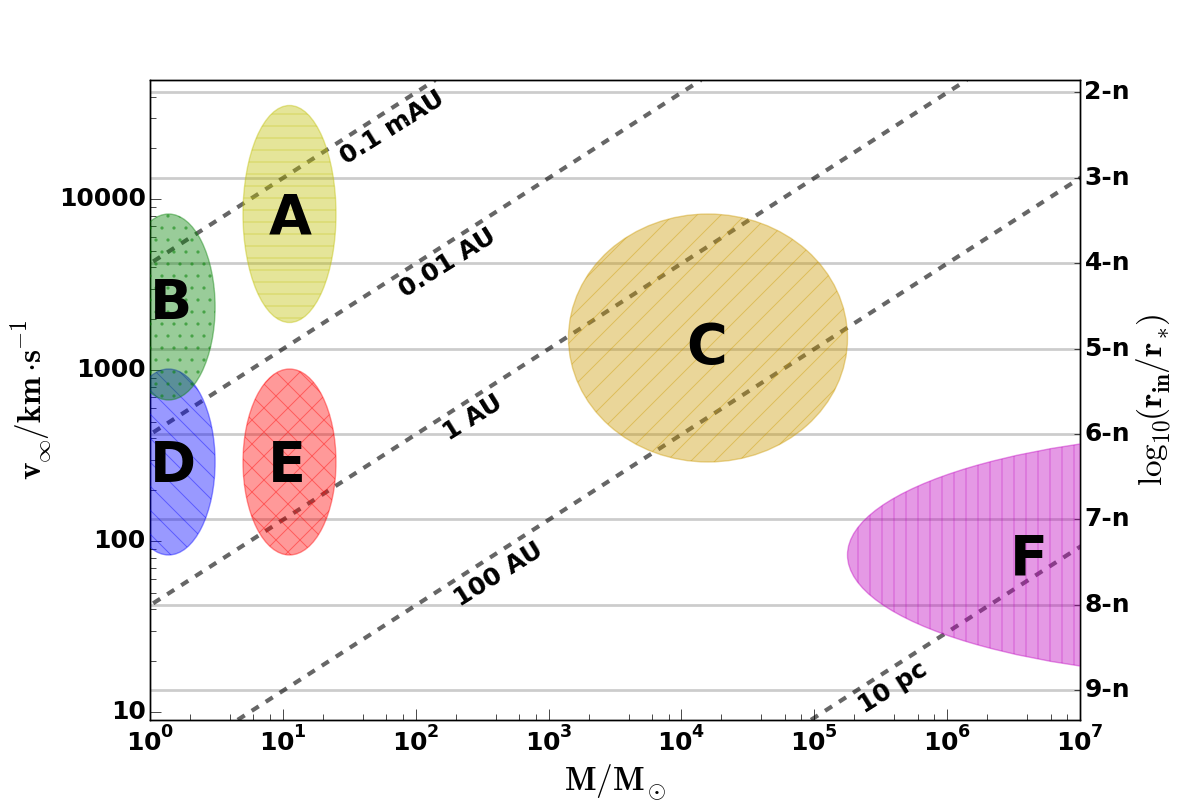
\includegraphics[width=0.8\textwidth]{dimensions_odm.png}
\caption{Contour map of the accretion radius as a function of the velocity at infinity and of the mass of the accreting body, confronted to an estimate of the computational cost on the right. The latter is represented by the ratio of the inner boundary radius $r_{in}$ by the Schwarzschild radius of the compact object $r_{*}$, with $n$ being given by $\zeta_{HL} / r_{in} = 10^n$, such as for n$=$0, the right axis indicates the physical ratio $\zeta_{HL} / r_{*}$. The coloured regions locate families of accreting compact objects (high and low mass X-ray binaries, intermediate and supermassive black holes, etc).}
\label{fig:dimensions_odm}
\end{center}
\end{figure}

We have been able to characterize the dependency of the mass accretion rates with the size of the inner boundary and to reach inner boundary sizes small enough to make the flow converge towards a given steady-state, an example of which being given at large (left) and small scales (right) by Figure\,\ref{fig:zoom}. We have witnessed for the first time the anchoring of the sonic surface into the accretor, a topological property derived by \cite{Foglizzo1996}. It is a strong consistency check which supports the robustness of those results.


\begin{figure}[ht!]
 \centering
 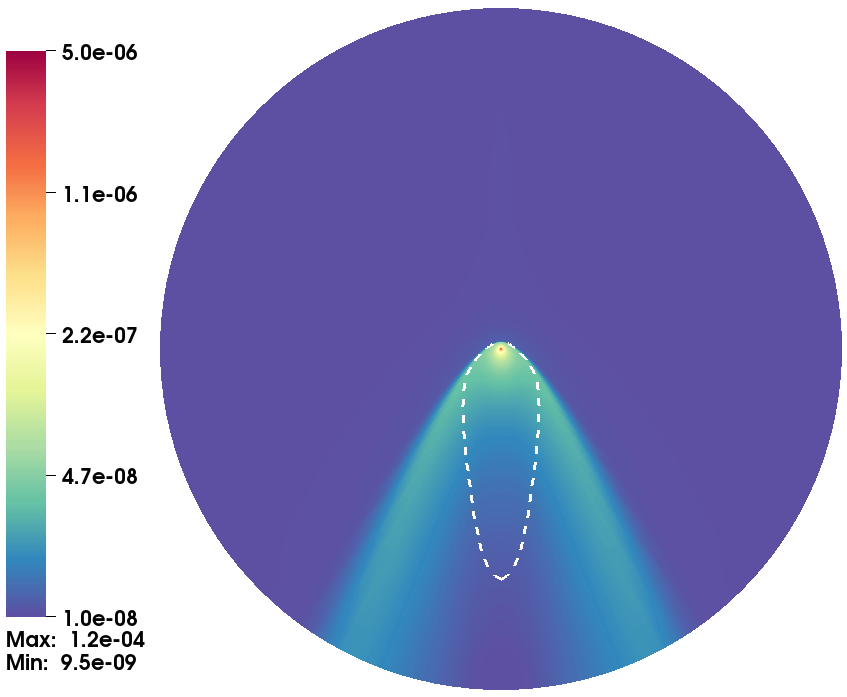
\includegraphics[width=0.46\textwidth,clip]{M040.png}%     
 \hspace*{2cm} 
 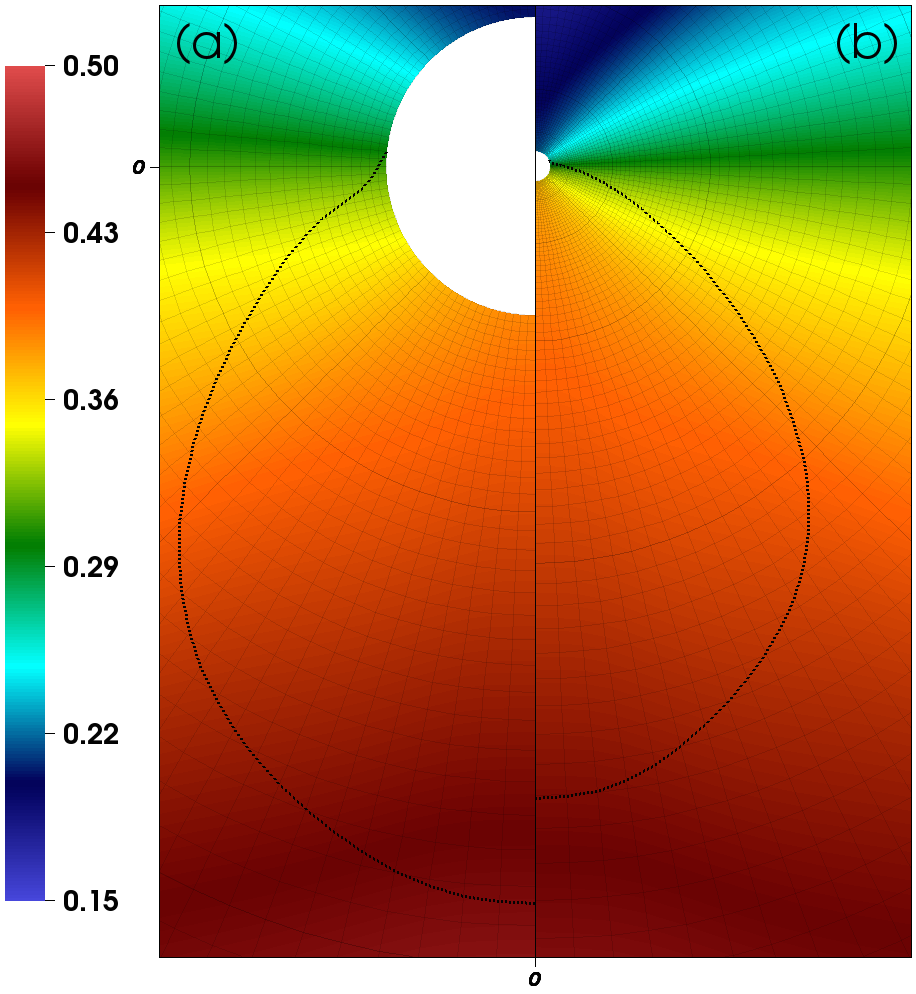
\includegraphics[width=0.33\textwidth,clip]{sonic_surface_different_inner_boundary_size.png}  
%% Note the ABSENCE of the extension .pdf  !
  \caption{Logarithmic colour map of the mass density of the flow for a Mach number at infinity of 4 (left panel) and a zoom in (by a factor of 400) on the inner zone (right). On the latter plot has been represented in color the local mass accretion rate. The dotted black line is the sonic surface, anchored in the accretor, whatever its size.}
  \label{fig:zoom}
\end{figure}

In parallel, we also started to relax the axisymmetric assumption of our 2.5D setup by running full 3D test-simulations of Roche-lobe overflow configurations, a snapshot of which can be seen on the snapshot below. 

\begin{figure}
\begin{center}
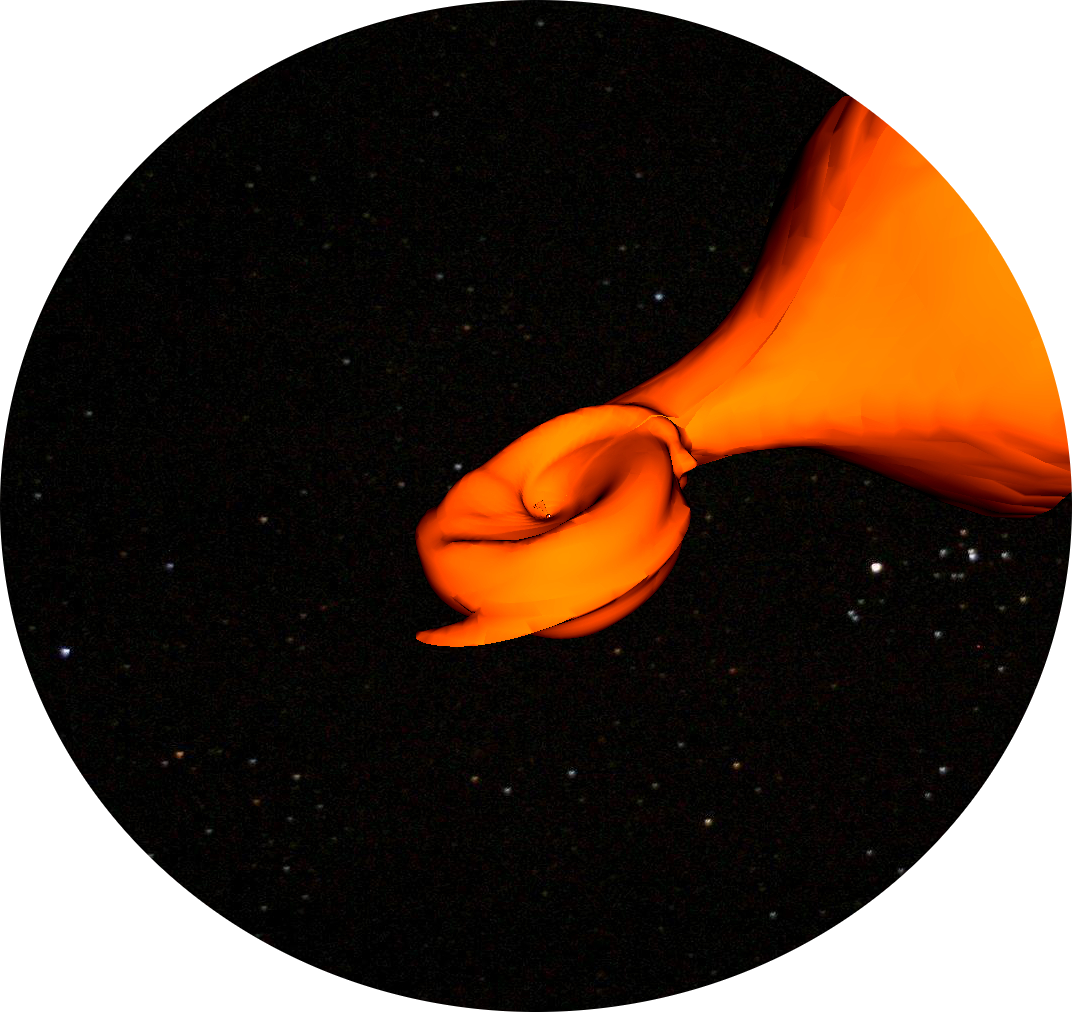
\includegraphics[width=0.3\textwidth]{RLOF_2.png}
\label{fig:RLOF}
\end{center}
\end{figure}

\vskip 0.5cm

\rubrique{Publications en pr\'eparation}
\vskip 0.2cm


\rubrique{Publications}
\vskip 0.2cm
\noindent \textit{Numerical simulations of axisymmetric hydrodynamical Bondi-Hoyle accretion on to a compact object} by I. El Mellah and F. Casse - Monthly Notices of the Royal Astronomical Society 2015 454 (3): 2657-2667 (doi: 10.1093/mnras/stv2184)



\rubrique{Conf\'erences et posters}
\vskip 0.5cm

\noindent Talk at the Journ\'ees de la SF2A (Soci\'et\'e Fran\c caise d'Astronomie et d'Astrophysique), Toulouse - June 2015\\  
\\
Invited talk at the COAST (COmputational ASTrophysics) meeting at the SAp (Service d'Astrophysique), CEA of Saclay - October 2015\\ 
\\
Poster at the 28$^{th}$ Texas symposium, Geneva - December 2015

\vskip 0.5cm



%\bibliographystyle{unsrt}


%\begin{thebibliography}{1}

%\section{Bibliographie}
%\label{Sec:Biblio}
\bibliographystyle{plainnat}
\bibliography{/Users/ielm/Documents/Bibtex/article_bhl_25D_no_url}

%\end{thebibliography}

\end{document}
%%%%%%%%%%%%%%%%%%%%%%%%%% Fin du fichier Latex %%%%%%%%%%%%%%%%%%%%%%%%%
